% Copyright 2006 Joshua LeVasseur <jtl@ira.uka.de>
%
% vim:textwidth=70
%

\documentclass[10pt,a4paper]{article}
\usepackage{graphicx}
%\usepackage{url}
\usepackage[pdftex]{hyperref}
\usepackage{times}

\typeout{dimension: textwidth	\the\textwidth}

\newcommand{\mytitle}{The L4Ka Afterburner Framework}
\newcommand{\myname}{Joshua LeVasseur}
\newcommand{\mysubject}{A developer's guide to the Afterburner and
components, on the L4 microkernel.}

\newcommand{\code}[1]{\texttt{#1}}
\newcommand{\cmd}[1]{\texttt{#1}}
\newcommand{\dir}[1]{\texttt{#1}}


\hypersetup{
  colorlinks=true,
  pdftitle=\mytitle,
  pdfauthor=\myname,
  pdfsubject=\mysubject,
}
\pdfpagewidth=\paperwidth 
\pdfpageheight=\paperheight 
%\pdfinfo {
%  /Title (\mytitle)
%  /Author (\myname)
%  /Subject (\mysubject)
%}

\title{\mytitle}
\author{\myname}

\raggedbottom

\begin{document}
\maketitle
\tableofcontents

\section{Change History}

\subsection*{7 September 2006}

Device-driver reuse is now ready for use by other developers
(supporting Linux 2.6.8.1).  I've
added a small section to this manual that should help you get started
configuring, building, and running a driver-reuse system.  See
\autoref{sec:driver-reuse}.

I've added several more configuration variables to the
wedge, regarding driver pass through.  You may need to reconfigure your
wedges.

I've also updated the Linux 2.6.8.1 patch, for statically linking
against driver reuse Linux modules.  If you want to use other Linux
versions, you'll have to update their patches to conform to the Linux
2.6.8.1 patch.

\subsection*{4 September 2006}

\begin{description}

\item[PCI forwarding:] The wedge has never had
true device pass through access, because some devices must be
virtualized by the hypervisor itself.  I've just added the ability to
partially virtualize the PCI bus too.  Currently the pass through is
enabled for a single PCI device on bus 0, which the guest OS will
discover as it scans the bus.  In the physical space, the device will
likely exist on a different bus; the virtual PCI topology differs from
the physical.  See \autoref{fig:pci_forwarding} for an example of PCI
topology remapping.

\begin{figure}[tb]
  \centering
  \includegraphics{figures/PCI-forwarding.pdf}
  \caption[PCI forwarding.]{We enable selective device pass through,
  and thus virtualize the PCI bus to avoid undesired device pass
  through.  Where pass through is desired, we forward the PCI requests
  from the virtual bus to the driver that handles the physical bus.
  The topology of the virtual bus is independent of the physical bus
  topology.}
  \label{fig:pci_forwarding}
\end{figure}


\item[OS bypass:] We run Linux kernel modules that are aware of the
wedge and of L4.  They often start L4 threads within the Linux kernel,
permitting interaction with other L4 entities, even outside of a valid
Linux context (OS bypass).  These threads are prohibited from directly
interacting with Linux internals, which is a problem when they raise
page faults.  One type of page fault that they can raise is due to an
unsynchronized page directory, which is missing a page directory entry
for the data and code executed by the L4 thread.  The Linux kernel
normally handles such faults by copying a page directory entry from
the master page directory into the active page directory.  It would be
rather complicated to generate a valid Linux context to permit the
Linux kernel to perform its fault handling, so I've modified the wedge
to emulate the synchronization.  Now a Linux kernel module is supposed to
register the Linux master page directory with the wedge, and then the
wedge will read mappings out of the master table if an L4 thread
raises a fault.  It is undesirable to add this intimate knowledge of
Linux into the wedge --- in the future we should find a different
solution.

\end{description}

I have changed configuration variables in several places; it may be
necessary to regenerate configurations via \code{make config}.


\subsection*{30 August 2006}

\begin{description}

\item[Wedge memory layout:] For initial bringup, the wedge was given fixed
physical and virtual memory allocations, which were specified via \cmd{make
config}.  The long-term goal is to make the wedge tiny and possible to fit
within a normal BIOS region.  I've moved towards that goal by removing the
fixed memory allocations --- I instead derive the size of physical memory from
the built-in ELF \code{\_end} symbol, while padding that region with a bubble
for additional dynamic allocations, with the bubble determined by \cmd{make
config}.  The command line argument \code{wedgesize=} is now obsolete.

Ramifications: \begin{description}
\item[Wedge:] You must rerun \cmd{make config} on all of your wedges, 
  to generate new configuration variables.
\item[\code{hypervisor\_idl.idl}:] This IDL file has changed, and thus
  all of its dependencies must be rebuilt.  This involves nearly everything
  related to L4: the resource monitor, device drivers, the wedge, command line
  utilities, etc.
\item[GRUB menu file:] You can remove the obsoleted \code{wedgesize=} parameter.
\end{description}

\item[Time-based sampling:] I've updated the resource monitor's
capabilities for sampling page working sets over time, and the
performance counters over time.  The sampling takes place via an L4
thread, and thus has high overhead compared to an in-kernel solution.
I've added two command line utilities (currently in
\dir{l4ka-driver-reuse/apps}) that start the sampler.  The sampler
prints its output to the debug console, in CSV format.  I cut-n-paste
the output into a text file, for processing by
\href{http://www.r-project.org/}{R}.  See
\autoref{fig:working_set} for an example.

\begin{figure}[tb]
  \centering
  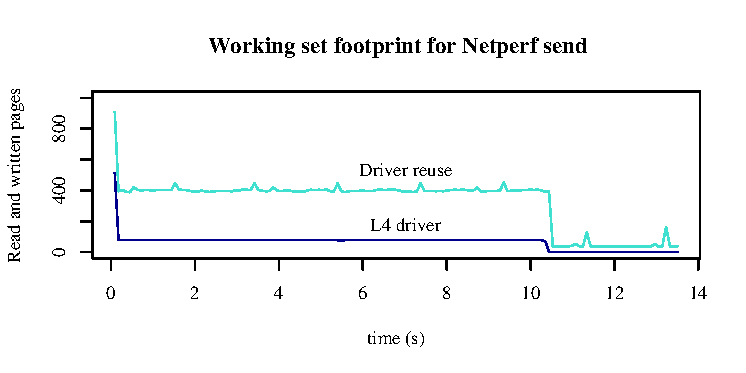
\includegraphics{figures/ws_netperf_send.pdf}
  \caption[Time plot of working set footprint for Netperf send.]{The
    working set footprint of the network device driver during Netperf send, 
    versus time, sampled at 90 ms intervals.}
  \label{fig:working_set}
\end{figure}

\item[Integrated resource monitor:] Until now, we've been using the Marzipan
resource monitor, developed to bringup the original L4Ka::Linux.  I have
created a fork of Marzipan within the Afterburner source tree, now called the
\emph{resource monitor}.  It resides in the subdirectory
\dir{l4ka-resourcemon}.  I updated it to use \cmd{make config}.  I
additionally created a fork of the IDL interface files, now within the
subdirectory \dir{l4ka-interfaces}.  The \cmd{make world} script
will automatically build the resource monitor.

Ramifications: \begin{description}
\item[IDL files:] All components
that import interface files now are configured to use the wrong files
(from the old Marzipan source tree).  The \cmd{make world} script
will automatically configure all components to use the new location,
but only if the old configurations are first removed.
\item[Runtime:]
If you experience bugs, it might be because you are mixing components
that use the old and new interface files.
\end{description}

\end{description}

\subsection*{24 August 2006}

Added a primitive data-space manager to the wedge, to handle page
faults in non-Linux code.  For example, a Linux kernel module could
accept L4 memory mappings, which later raise page faults.  By installing a
data-space handler, the module can resolve the page fault.  The
data-space handler runs in the context of the L4 pager thread, and
thus \emph{must not interact with Linux internals}.  I'm currently
using the data-space handler for the block driver's shared pages.

\subsection*{18 August 2006}

\code{printf()}: Due to popular demand, I've added \code{printf()}
to the Afterburner wedge.  It is 64-bit broken.  But I've upgraded
\code{printf()} in the resource monitor to be 64-bit clean.

\subsection*{17 August 2006}

Linux 2.6.8.1: The old L4Ka::Linux is actually 2.6.8.1, not
2.6.9.  Thus for performance comparisons between para- and pre-
virtualization, I've added a Linux 2.6.8.1 patch.  It is now the most
up-to-date patch.

\subsection*{16 August 2006}

Added a native L4 device driver for the e1000 network adapter.  The
driver is fast, but is built for benchmarking, and thus has several
deficiencies.  The driver is located in the \dir{l4ka-driver-native}
subdirectory.

\subsection*{31 July 2006}

Added a comprehensive profiler to the wedge and to Linux, as an
alternative to gprof.  A disadvantage of gprof is its overhead, since
it relies on dynamic memory, dynamic data structure lookups, and
function calls.  My alternative takes advantage of gcc's preparation
for gprof (such as saving and restoring registers), but replaces the
gprof invocations with high-performance code, by Afterburning the
source code.  The Afterburner locates all function calls to gprof, and
replaces each instance with static memory allocation of a profile counter,
along with a single instruction to increment the counter.

I also added infrastructure for basic wedge system calls, so that a
Linux application can invoke a method within the wedge.  I use this
framework for retrieving the profile results, to store to disk.  I
wrote an ELF parser to correlate the profile results with
function names.  The utilities are located in the \dir{wedge-apps}
subdirectory.

\subsection*{12 July 2006}

Added a new item to the soft layer to handle faults caused by the wedge
when it accesses user memory.  This item is a Linux
\code{exception\_table\_entry}, which contains the instruction address
of a potential faulting instruction, and the instruction address of a
handler routine that takes control in the event of a fault, receiving
full register contents of the faulting instruction.  The wedge has
many places that access user memory, but needs only one
\code{exception\_table\_entry}, because the entry is used during page
fault handling, and the wedge has a single fault handler.


\section{Build Infrastructure}

Each subproject has a dedicated Make environment that permits the
project to be built independently from the remaining subprojects.  A
top-level Make environment combines together all of the subprojects via
recursive make invocations.

The build environments have been evolving as I've added subprojects.
The latest environment, with my preferred approach and to be used as
templates for new subprojects, are in the \dir{l4ka-driver-native} and
\dir{l4ka-resourcemon} subprojects.

The key criteria of these model build environments are that they:
\begin{itemize}
\item permit building the projects in build directories separate from
the source directories;
\item use a configuration utility that can ensure integrity of the
configuration variables (currently I use CML2);
\item automatically calculate dependencies between source files, to
ensure that all dependencies of a modified file are also rebuilt.
\end{itemize}

Additionally, I have come to prefer storing header and source files
within the same directory, rather than dividing them different
directories.  This provides quick access to header and source pairs
while editing, and avoids large collections of header files within a
single directory.


\section{Device Driver Reuse}
\label{sec:driver-reuse}

I provide the ability to \emph{reuse} Linux device drivers for block
and network devices, by running the original device drivers within a
virtual machine, supported by their original Linux kernel.  To share
the devices, you load Linux kernel modules into the device driver VMs,
which translate between internal Linux device operations and external
L4 device requests.  From this perspective, the driver VM is the L4
server, and the other L4 processes are clients.  For an in-depth
description, refer to our
\href{http://l4ka.org/projects/virtualization/drivers.php}{publications}.
Also see \autoref{fig:driver_translation_module} and
\autoref{fig:driver_isolation}.

To enable the client virtual machines to access the devices, you
install para-virtualized device drivers for accessing the block and
network devices, or may use the pre-virtualized DP83820 network device
model to access reused network devices (see
\autoref{fig:previrtualized_PCI} and
\autoref{fig:previrtualized_network}).

The driver reuse is experimental, and lacks features expected from a
production environment, particularly error handling, resource release,
and easy configuration.

You can run all reused drivers within a single VM, or run them within
separate VMs for device driver isolation.  The isolation increases
complexity, since you must configure and build multiple VMs, and run a
PCI VM to handle the shared PCI bus.

\begin{figure}[tb]
  \centering
  \includegraphics{figures/translation-module.pdf}
  \caption[Translation module for driver reuse.]{Drivers execute
  within their native OSes, within a VM.  We install translation
  modules into the driver OS for enabling driver access by other L4
  processes.}
  \label{fig:driver_translation_module}
\end{figure}

\begin{figure}[tb]
  \centering
  \includegraphics{figures/isolated-drivers.pdf}
  \caption[Isolated, reused drivers.]{Each driver executes within
  its native OS, within a VM.  We install a translation
  module into each driver OS for enabling driver reuse.  The
  architecture is recursive --- the driver VMs can reuse drivers from
  other driver VMs, such as a shared PCI bus driver.}
  \label{fig:driver_isolation}
\end{figure}

\begin{figure}[tb]
  \centering
  \includegraphics{figures/previrtualized-PCI.pdf}
  \caption[Reused PCI driver with a pre-virtualized client OS.]{We use
  pre-virtualization to quickly build virtualized device models.  In this
  example, we have built a PCI virtual device, which permits a driver
  OS to access the shared PCI bus.}
  \label{fig:previrtualized_PCI}
\end{figure}


\begin{figure}[tb]
  \centering
  \includegraphics{figures/previrtualized-network.pdf}
  \caption[Reused drivers with a pre-virtualized client OS.]{We use
  pre-virtualization to build high performance device models.  In this
  example, we have a high-performance DP83820 model that obtains
  network services from a reused network driver.}
  \label{fig:previrtualized_network}
\end{figure}



\subsection{Wedge Configuration}

You will use different wedge configurations for the driver VMs and the
client VMs.  The driver VMs require device pass through, which must be
enabled via the wedge's \cmd{make config} command:  \begin{itemize}
\item If you use a composite driver VM that handles all devices, then 
you can enable full device access.
\item If you will isolate drivers in multiple VMs, then
you want to selectively enable device access, and use PCI forwarding.
The PCI forwarding sends PCI requests for the VM's device to a
PCI-driver VM.  You must hard code the configuration for the PCI
forwarding, i.e., the identify of the device for which to forward PCI
requests.  The identity includes the PCI vendor and device IDs.
For the PCI-driver VM, you enable PCI bus pass through as opposed to
PCI forwarding.
\end{itemize}


\subsection{Building Linux Driver Reuse Modules}

Device driver reuse adds many additional components to your system,
and thus more configuration, build, and management complexity.  I've
automated most of the hassle within the \cmd{make world}
infrastructure.  The following sections describe how to take advantage
of my driver reuse, whether you use the \cmd{make world} automation,
or handle the steps yourself.

Note that I have tested this only with Linux 2.6.8.1.  The Afterburner
patches for other Linux versions are probably outdated.

\subsubsection{Link}

Link the driver reuse project into the Linux 2.6 source
tree, so that you can either build loadable modules, or statically link
the modules into your Linux kernel binary.  If you use the automated \cmd{make
world} script, then you need only execute \cmd{make prereqs-linux-2.6}
from your Afterburn build directory (I would like to automate this step, but it
introduces an ordering problem to Make, and thus you must execute it
manually).  If you are building things manually without the help of
the \cmd{make world} script, then execute the following steps:
\begin{enumerate}
\item Link the \dir{l4ka-driver-reuse/kernel} subdirectory into
the Linux source tree as \dir{afterburn/drivers}.
\item Add the driver reuse configuration system to the Linux 2.6
configuration system.  Add the line 
\begin{verbatim}source "afterburn/drivers/Kconfig"\end{verbatim}
to the bottom of the \dir{afterburn/Kconfig} file.
\end{enumerate}

\subsubsection{Configure}
\begin{enumerate}
\item Enable driver support within Linux's configuration system, by
executing Linux's \cmd{make config} system.  If you use the automated
\cmd{make world} script, then you can execute \cmd{make
reconfig-linux-2.6-\emph{name}} from the Afterburn build directory.
Go to the \emph{Afterburn Driver Reuse} configuration menu, and then
enable driver reuse, and choose the type of modules to
build (the server translation modules or the client para-virtualized
drivers), and whether to make them static or dynamic
modules.  If you use the DP83820 interface for the network client, be sure to
enable your DP83820 device within the Linux kernel.  Currently, your
network server can either support the DP83820 interface, or the
para-virtualized network interface, but not both simultaneously.
\item You must tell it the name of your wedge binary, because the
Linux build process will import absolute symbols from the wedge.  This
requires you to rebuild Linux each time you rebuild the wedge.  In the
future, we hope to add dynamic symbol resolution against the wedge
(which I already support for dynamically loaded Linux modules, but not
for a static Linux kernel binary).  The name is a suffix of the
wedge's name, where the suffix uniquely differentiates a wedge from
other wedge configurations.
\item If you are avoiding the \cmd{make world} automation, then you
have an additional manual step.  In your Linux build directory,
create a file called \dir{afterburn/drivers/cfg.Mk}, and in it,
define the following Make
variables: \begin{itemize}
\item \code{cfg\_pistachio\_dir} - The directory containing the
user-level Pistachio files, i.e., where to find \dir{include/l4}.
\item \code{cfg\_wedge\_build\_prefix} - The prefix of the wedge
binary.  It is combined with the suffix, specified earlier, to form a
full path to the wedge binary.
\item \code{cfg\_marzipan\_dir} - The interfaces directory, i.e., the
path of the \dir{l4ka-interfaces} directory.
\end{itemize}

\end{enumerate}


\subsubsection{ROM for Loadable Modules}

The \cmd{make world} script will automatically generate a ROM image
for Linux, which contains the translation modules, and an init process
to load the translation modules.  The init process is designed for use
in the driver server VM --- after loading the translation modules, it
sleeps forever, thus making a low-overhead VM that executes no
user-level services.

To build driver ROMs for all of your Linux configurations that have
enabled driver reuse, execute \cmd{make install-l4ka-driver-reuse}.
This step will automatically download and install the utilities needed
for generating a ROM, along with Linux's module management utilities.
Additionally it downloads a light-weight C library, used for all
utilities loaded from the ROM.

\subsection{GRUB Configuration}

Driver reuse requires you to load serveral more modules at boot time
via GRUB.  

The following example loads a composite driver-reuse VM, along
with the special ROM for initializing the VM.  It then loads a second
VM that reuses the devices.
\begin{footnotesize}
\begin{verbatim}
title = Composite driver reuse
kernel = (nd)/tftpboot/joshua/auto/kickstart
module = (nd)/tftpboot/joshua/auto/pistachio
module = (nd)/tftpboot/joshua/auto/sigma0
module = (nd)/tftpboot/joshua/auto/l4ka-resourcemon
module = (nd)/tftpboot/joshua/auto/afterburn-wedge-l4ka-passthru vmstart \
        ddos vmsize=20M wedgeinstall=16M
module = (nd)/tftpboot/joshua/auto/vmlinuz-2.6.8.1-i30pc30-ddos \
        root=/dev/ram0 \
        init=/l4ka-drivers-init ro console=tty console=ttyS0,115200
modulenounzip = (nd)/tftpboot/joshua/auto/rom-driver-reuse-2.6.8.1-i30pc30-ddos-vdev.gz
module = (nd)/tftpboot/joshua/auto/afterburn-wedge-l4ka-guest vmstart \
        vmsize=256M wedgeinstall=16M
module = (nd)/tftpboot/joshua/auto/vmlinuz-2.6.8.1-i30pc30-guest \
        console=tty console=ttyS0,115200 ramdisk_size=32768 \
        root=/dev/ram0 init=/sbin/init rw devfs=mount \
        ip=10.30.0.1:10.30.0.1:10.30.0.1:255.0.0.0:i30pc30:eth0:off \
        blockprobe=8,6
module = (nd)/tftpboot/joshua/auto/perfmon-ramdisk.img.gz
\end{verbatim}
\end{footnotesize}

The wedge used for driver reuse has a special command-line option: \code{ddos}.
This tells it to prepare for performing indirect DMA with other VMs.  I've
allocated it a 20MB VM.


\section{QEMU}

\href{http://fabrice.bellard.free.fr/qemu/user-doc.html}{QEMU} is a
whole-machine emulator, useful for operating system development and
testing.  The \cmd{make world} script will retrieve, patch, and build
QEMU for you.  

\subsection{Patch Description}

The patch improves support for Mac OS X (although it doesn't fix
key-binding problems when using the graphics console device, nor does
it enable support for Mac OS X 10.4\footnote{Mac OS X 10.4 broke the
\code{poll()} system call, which QEMU uses for its event loop, thus
breaking QEMU's serial console.}).  The patch additionally makes the
built-in tftp server more portable between machines, by removing
support for paths in tftp requests.  Instead, the tftp server converts
all file requests, no matter the path, into requests for files from
the current working directory of QEMU.  Doing so permits a single GRUB
configuration to simultaneously support real hardware (and a real tftp
server), and QEMU.  But more importantly, it permits a prebuilt boot
floppy image to work within your environment --- the automated build
script will retrieve a boot floppy from the L4Ka.org web site, which
already contains a GRUB boot sector configured to contact QEMU's tftp
server to retrieve a \dir{menu.lst} file.

\subsection{Execution}

To execute QEMU, change into your build directory and execute
\cmd{make run-qemu}.  If your boot directory (as recognized by the
automated build script) doesn't contain a GRUB \dir{menu.lst} file,
the automated build script will generate an example file.  And
additionally, the automated build script will fetch a GRUB boot
floppy, called \dir{qemu-afterburner-floppy.img}, from the L4Ka.org
web site.  This file enables you to immediately use QEMU, without
having to create a real hard disk image.  Of course, without a hard
disk image, and without a RAM disk image, Linux will only partially
boot.

The \cmd{make run-qemu} command chooses QEMU's most portable settings.
It disables graphics.  It uses user-level networking (and attempts to
tie the host port 3022 to the guest OS at port 22 for ssh, and assumes
that you configure your guest OS to use IP address 10.0.2.10).  Since
it disables the graphics support, it attaches the current terminal to
the virtual serial port.  Thus if you configure your guest OS to use
the serial console, then the booting kernel will send its boot
messages to the current terminal, and will open a login prompt at the
current terminal.  And if any of the virtualization environments
support an interactive debugger, then it can be activated from the
current console.  The L4Ka::Pistachio kernel often uses the
\cmd{Escape} key to activate the kernel debugger.  My Mac OS X
terminal can send an \cmd{Alt-F} keystroke to trigger a serial port
break, for entering the kernel debugger.  The KaXen wedge uses
\cmd{Ctrl-x} to activate the debugger.  QEMU has a command console,
activated by pressing \cmd{Ctrl-a}, followed by \cmd{c}. The Xen
hypervisor uses three successive presses of Ctrl-a to activate its
debug console, which interferes with QEMU, and so is actually enabled
by pressing \cmd{Ctrl-a} followed by \cmd{a}, the whole pattern
repeated three times.

Note that the L4Ka environment is missing a console input driver,
which means you'll have to connect to the VM over the network for user
interaction.

If everything works as planned, you should be able to retrieve the
Afterburn project from CVS, execute \cmd{make world}, and then execute
\cmd{make run-qemu}, and boot Linux to the point where it tries to
mount a root disk.  The error message will be:

\begin{footnotesize}
\begin{verbatim}
VFS: Cannot open root device "<NULL>" or unknown-block(0,0)
Please append a correct "root=" boot option
Kernel panic - not syncing: VFS: Unable to mount root fs on unknown-block(0,0)
\end{verbatim}
\end{footnotesize}

\subsection{Configuration}

The \cmd{make world} script automatically generates the GRUB menu
\dir{afterburn.lst} in your boot directory.  The script will likely
surprise you by overwriting any changes that you make to that file, so
instead, maintain your custom configuration in a new file.  You can
easily tie your new file into the GRUB menu system by adding an entry
to the \dir{menu.lst} file in your boot directory.  Here is an example
\dir{menu.lst} file, which points to a custom GRUB menu file named
\dir{qemu.lst}:

\begin{footnotesize}
\begin{verbatim}
serial --unit=0 --speed=115200
terminal serial console
default 0

title = QEMU stuff
configfile = (nd)/tftpboot/afterburn/qemu.lst

title = Afterburn Stuff
configfile = (nd)/tftpboot/afterburn/afterburn.lst
\end{verbatim}
\end{footnotesize}

Here is an example GRUB menu that loads a RAM disk, and configures the
networking from the kernel command line (which avoids hard coded
network configuration in the RAM disk, and avoids inefficient kernel
support for automated configuration via DHCP):

\begin{footnotesize}
\begin{verbatim}
title = L4Ka (device passthru)
kernel = (nd)/tftpboot/afterburn/kickstart-serial
module = (nd)/tftpboot/afterburn/pistachio-qemu
module = (nd)/tftpboot/afterburn/sigma0-serial
module = (nd)/tftpboot/afterburn/l4ka-resourcemon
module = (nd)/tftpboot/afterburn/afterburn-wedge-l4ka-passthru \
         vmstart vmsize=128M wedgeinstall=16M
module = (nd)/tftpboot/afterburn/vmlinuz-2.6.9-qemu  \
         console=tty console=ttyS0,115200 root=/dev/ram0 rw \
         ramdisk_size=32768 \
         ip=10.0.2.10:10.0.2.2:10.0.2.2:255.255.255.0:minime:eth0:off
module = (nd)/tftpboot/afterburn/ramdisk.img.gz

title = Afterburnt Linux on raw hardware
kernel = (nd)/tftpboot/afterburn/bzImage-2.6.9-qemu \
        console=tty console=ttyS0,115200 root=/dev/ram0 rw \
        ramdisk_size=32768 \
        ip=10.0.2.10:10.0.2.2:10.0.2.2:255.255.255.0:minime:eth0:off
module = (nd)/tftpboot/afterburn/ramdisk.img.gz
\end{verbatim}
\end{footnotesize}


\end{document}
